\chapter{Prozess Anforderungen}
Da die Software Architektur auf den Anforderungen basiert und viel wichtiger \glqq den gestalterischen Spielraum des Architekten\grqq \cite[S. 103]{softarch} begrenzt, kann davon abgeleitet werden, dass sowohl die Qualität der Architektur als auch die Akzeptanz des Systems wesentlich von den bereits im Vorfeld ermittelten Parametern abhängt. Das bedeutet wiederum, dass für die Klärung der Ausgangsfrage - Wie kommt man von Anforderungen auf eine gute Architektur - auch der Anforderungsprozess eine wichtige Rolle spielt.

Da der Anforderungsprozess ein an sich eigenes, sehr großes Themengebiet dar stellt, wird hier jedoch nur auf die Ausgangsartefakte eingegangen, welche später im Architekturprozess referenziert werden.

Die Entwicklung der meisten Software Projekte ist oft ein dynamischer und agiler Prozess. Während des Entwicklungsprozesses werden oft Änderungen eingebracht und neue Anforderungen aufgestellt  \cite[S. 6-7]{effektiv}. Auch führt die Komplexität des Systems und das Wissen des/der KundIn dazu, dass nach der Erhebung der initialen Anforderungen nicht alle Parameter vollständig bekannt sind. Dies wiederum führt mehr oder weniger dazu, dass der Anforderungsprozess während der Entwicklung der Architektur nicht als abgeschlossen gesehen werden kann und der/die KundIn verfügbar sein muss. Dieses scheinbare Problem erlaubt es jedoch, den Aufwand der Aufnahme bestimmter Anforderungen zu minimieren, da bereits viele Kombinationen ausgeschlossen werden können.

\section{Ermittlung der Usecases}
Die Usecases werden zusammen mit dem/der Kundin ermittelt. Daraus wird schlussendlich ein Usecase Diagramm erstellt, welches alle Akteure und Nebensysteme beinhaltet. Dies ist wichtig für das Kontextdiagramm, welches auch im Anforderungsprozess erstellt wird und die Ausgangsbasis für die Architektur dar stellt.

\begin{figure}[!htbp]
    \centering
    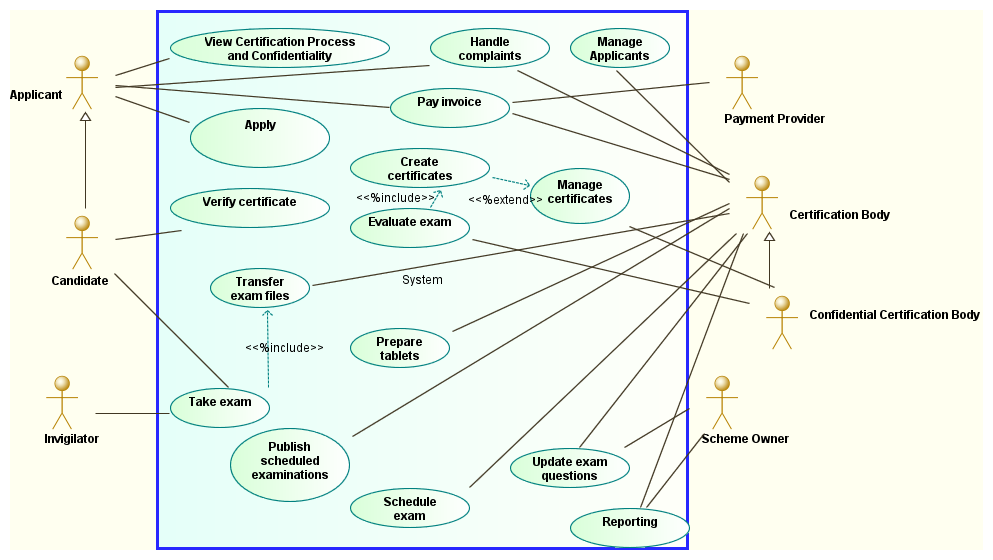
\includegraphics[scale=0.4]{uml/usecase.png}
    \caption{Das mit dem Kunden ermittelte Usecase Diagramm}
\end{figure}

\subsection{Erweiterte Dokumenation der Usecases}
Parallel zur Erstellung des Usecase Diagramms werden zusätzliche Parameter und Beschreibungen für jeden Usecase aufgenommen, welche im eigentlichen Diagramm keine Erwähnung finden.
Dafür wird ein Anforderungstemplate, auch Usecase Beschreibung genannt, verwendet \cite[S. 214]{reqman}, welches aufbauend auf einer Grundversion \cite[Abbildung 8.14, S. 215]{reqman} für jeden Usecase folgende Angaben aufnimmt:

\begin{itemize}
  \item Id: eine eindeutige Bezeichnung, welche dafür verwendet wird, um den Usecase zu referenzieren
  \item Actor: eine Auflistung aller Teilnehmer des Usecases
  \item Description: eine kurze Beschreibung des Usecases
  \item Preconditions: eine Auflistung von Vorbedinungen für den Usecase
  \item Postconditions: eine Auflistung von Nachbedingungen für den Usecase
  \item Normal Course of Events: eine Beschreibung des Standardablaufes
  \item Alternative Courses: Auflistung von Erweiterungen oder zusätzlichen Möglichkeiten
  \item Exceptions: Beschreibung von diversen Ausnahmefälle
  \item Assumptions: Annahmen, unter welcher der Usecase beschrieben wird
  \item Priority: eine Gewichtung, wie wichtig der Usecase ist
  \item Notes: sonstige Anmerkungen
\end{itemize}

Sind die Abläufe komplexer, können Aktivitäts Diagramme verwendet werden, um komplexere Abläufe verständlicher dar zu stellen \cite[S. 215]{reqman}:

\begin{figure}[H]
    \centering
    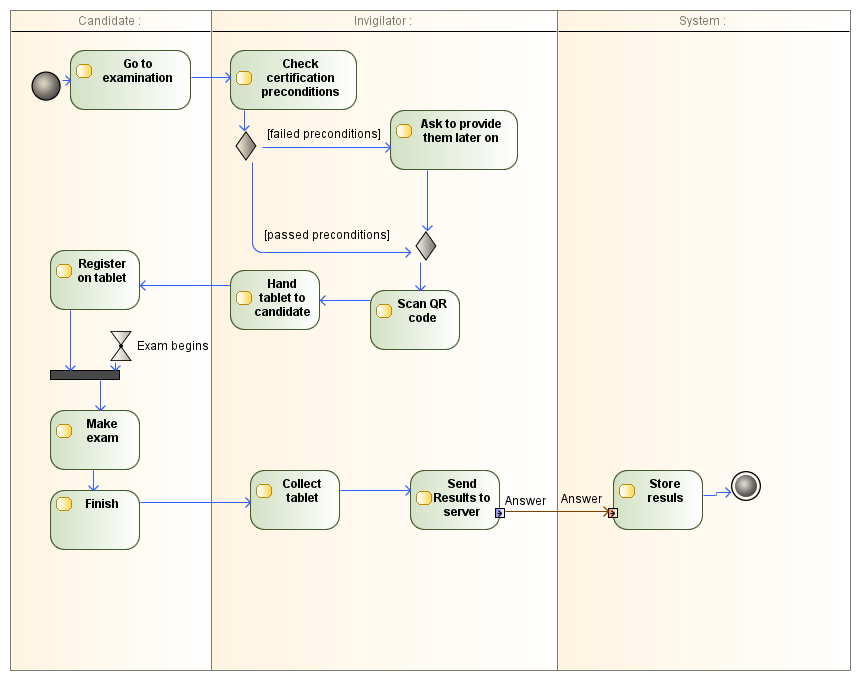
\includegraphics[scale=0.4]{uml/takeexamreq.png}
    \caption{Der Ablauf des Take Exam Usecases im Detail}
\end{figure}

\subsection{Einbeziehen von Architekturreviewparametern}
Um die Einhaltung der Qualitätsparameter zu garantieren, können Architekturreviews durchgeführt werden \cite[S. 20]{review}. Es existiert zwar \glqq keine singuläre, allgemein akzeptierte Metrik um eine Architektur zu beurteilen\grqq \cite[S. 19]{review}, jedoch liefern sie grobe Einschätzungen über die Angemessenheit des Systems \cite[S. 20]{review}. Folgende Architekturreviews wurden dafür ausgewählt:

\begin{itemize}
  \item ATAM: betrachtet Wachstums- und explorative Szenarien um die Architektur zu beurteilen \cite[S. 61]{review}
  \item CBAM: basiert auf ATAM, beachtet jedoch vor allem den Nutzen und die Risiken und Kosten der Architketur, um die Architekturentscheidungen besser abwähgen zu können. Hauptfaktor ist der ROI. \cite[S. 67]{review}
\end{itemize}

Für diese Reviews können bereits früh ein Großteil der benötigten Parameter ermittelt bzw. zumindest grob abgeschätzt werden. Dies ist wichtig, weil nach der 10er Regel der Fehlerkosten früh erkannte Fehler und Probleme weniger Kosten nach sich ziehen als später Erkannte \cite[S. 154]{fehler}.

Deswegen wird das Anforderungstemplate um folgende Parameter erweitert:

\begin{itemize}
  \item Earned Value per month: Wieviel Umsatz der Usecase in einer bestimmten Zeit generiert
  \item Expected Usage: Anzahl der erwarteten Nutzer des Systems pro Zeiteinheit
  \item Growth Scenarios: Anzahl der erwarteten Nutzer des Systems pro Zeiteinheit bei einer höheren Nutzeranzahl
  \item Change Scenarios: mögliche Änderungsszenarien und Erweiterungen
\end{itemize}

\subsection{Einbeziehen von nicht funktionalen Qualitätsattributen}
Nicht funktionale Qualitätsattribute beschreiben die nicht funktionalen Anforderungen an das System. Da Qualität oft schwammig formuliert ist, ist es wichtig, diese Attribute messbar zu machen \cite[S. 9]{effektiv}.

Deswegen werden für jeden Usecase und dessen architekturrelevanten, nicht funktionalen Anforderungen messbare Parameter definiert. Diese Parameter helfen schon im Vorfeld dabei die Architektur zu überprüfen.

Für das Beispielprojekt wurden folgende Parameter definiert, mit welchen das Anforderungstemplate erweitert wurde:

\begin{itemize}
  \item Response Time in Seconds: Wie schnell die Antwort des Systems auf eine Anfrage reagieren muss
\end{itemize}

\section{Rahmenbedingungen}
Zusätzlich zu funktionalen und nicht funktionalen Anforderungen werden auch die Rahmenbedingungen ermittelt, unter welchem das System erstellt werden soll. Diese Anforderungen beinhalten meist den organisatorischen und zeitlichen Ablauf des Projektes und können auch gewisse Technologien vorschreiben, zB. wenn das System in ein bereits bestehendes System integriert werden soll. \cite[S. 9]{review}\cite[S. 110]{softarch}

Die Rahmenbedingungen des Beispielprojektes lassen sich zum Großteil aus dem ISO Standard für Zertifizierungsstellen ermitteln \cite{ISO_CERT} und geben Einsicht in die Vertraulichkeit der Daten und eröffnen weitere Usecases. Sofern möglich werden diese Parameter in das Usecase Diagramm und das Klassen Diagramm der zu verwendeten Daten mit einbezogen. Auf zeitliche und technologische Rahmenbedingungen wurde im Beispielprojekt nicht eingegangen.

\section{Ermittlung der Daten}
Die verwendeten Daten werden ermittelt und mit Hilfe eines Klassen Diagrammes modelliert. Dies ist nicht nur wichtig und nützlich, weil die Beispielanwendung in diesem Falle eine stark datenzentrierte Anwendung ist \cite[S. 105]{effektiv}, sondern wird später auch einen wesentlichen Beitrag zur Aufteilung des Systems in Komponenten leisten. Im Falle des Beispielprojekts wurden folgende Daten ermittelt und modelliert:

\begin{figure}[H]
    \centering
    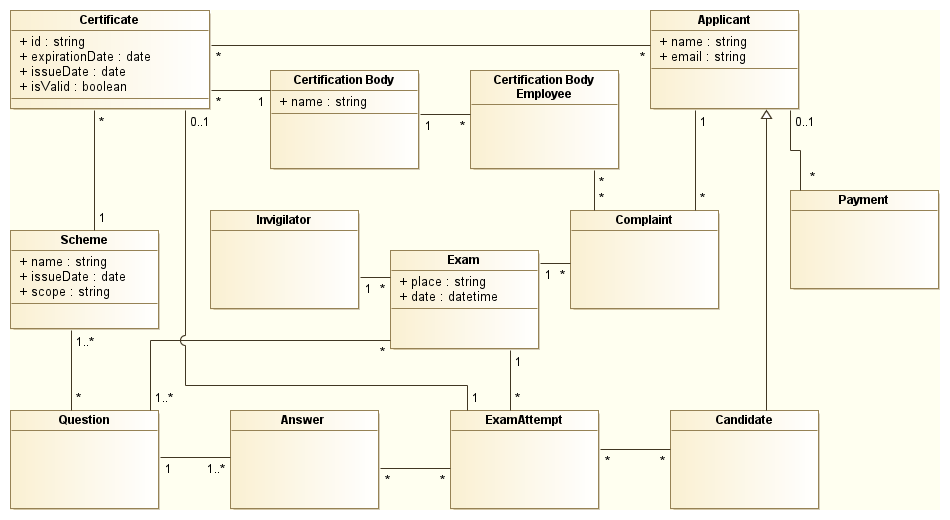
\includegraphics[scale=0.5]{uml/class.png}
    \caption{Das ermittelte Klassendiagramm des Beispielprojektes}
\end{figure}

\section{Ermittlung der Zonen}
Nach der Ermittlung der Daten wird auf Basis der Rahmenbedingungen und Sicherheitsstruktur zusammen mit dem/der Kunden/Kundin ermittelt, welche Zonen für das System benötigt werden. Zonen stellen eigene abgeschlossene Bereiche dar, in welchen das System operiert oder von welchem auf das System zugegriffen werden kann. Grundsätzlich existiert mindestens eine Zone. In diesem Fall beherbergt diese Zone das interne System des Unternehmens.

Soll von anderen Systemen, zB. vom Internet auf Funktionalitäten des Systems zugegriffen werden können, wird eine weitere Zone benötigt.

Aus den Usecases des Beispielprojektes lässt sich ermittelt das in diesem Falle mindestens zwei Zonen benötigt werden:

\begin{itemize}
  \item Public: Usecases die vom Internet auf das System zugreifen, zB. wenn sich ein Anwärter (Applicant) für eine Prüfung registriert
  \item Internal: Usecases, welche nicht vom Internet aus zugänglich sind
\end{itemize}

Die Zonen werden nun mit einer Vertrautheitsebene von 1 bis n versehen, um eine Sicherheitshirarchie der Zonen zu generieren. Es kann vorkommen, dass mehrere Zonen mit der selben Vertrautheitsebene versehen werden, diese dürfen sich jedoch nicht überlappen. Zum Beispiel könnte eine weitere Tocherniederlassung der Firma ein eigenes System erstellen, auf welches man auch vom Internet aus zugreifen kann. Das Internet würde dann mit der Vertrautheitsebene 1 versehen und beide Systeme mit der Ebene 2. Überlappen sich diese Systeme, muss die überlappende Zone in ein eigenes System ausgegliedert werden.

Die ermittelten Daten werden nun den Zonen, in welchen sie essentiell für den Betrieb des Systemes sind, zugeteilt. Auch die Akteure werden in Zonen aufgeteilt, in welchen sie operieren. Scheinen Daten oder Akteure in mehreren Zonen auf, werden sie der Zone mit der höchsten Sicherheitsebene zugeteilt. Die niedrigeren Bereiche können dann auf diese Bereiche anhand von festgelegten APIs zugreifen.

Im Falle des Beispielprojektes werden alle aufgenommen Daten in der Internal Zone verwaltet, da alle Daten als businesskritisch für das Internal System angesehen werden, welches wiederum die höchste Sicherheitsebene besitzt. Würde das Beispielprojekt zB. um ein Forum oder einen Blog erweitert, würden diese der Public Zone zugeteilt werden; AkteurInnen des Internal Systems können zwar auch auf diese Forum zugreifen oder Blogeinträge schreiben, jedoch sind diese Aktivitäten und Daten nicht kritisch für den normalen Betrieb des Internal Systems. Würde das Forum oder der Blog gehackt werden, resultiert dies zwar in einem Schaden für das Unternehmen, das Internal System könnte aber auch weiterhin normal operiert werden.

Nach der generellen Aufteilung der Daten wird eine Analyse der Rahmenbedingungen durch geführt, um zu erfahren, ob bestimmte Daten aufgrund von Richtlinien besonders geschützt, und somit in eine eigene Zone mit einer höheren Vertrautheitsebene ausgelagert werden müssen. Das Beispielprojekt verlangt die vertrauliche Verarbeitung von Prüfungsergebnissen und erwähnt auch explizit das Personal der Prüfungsstelle \cite[7.3]{ISO_CERT}. Weil die Internal Zone, in welchem das Personal operiert, die Zone mit der höchsten Vertrautheitsebene darstellt, muss eine weitere Zone mit einer höheren Vertrautheitsebene erstellt werden. Diese Zone wird in diesem Falle mit der Vertrautheitsebene 3 versehen und unter der Beschreibung Confidential geführt.

Um diese Zonen besser zu visualisieren zu können, wird das UML Metamodel mit Hilfe eines Profiles angepasst. Jede Zonen erhält einen gleich lautetenden Stereotypen \cite[S. 518]{glasklar}:

\begin{figure}[H]
    \centering
    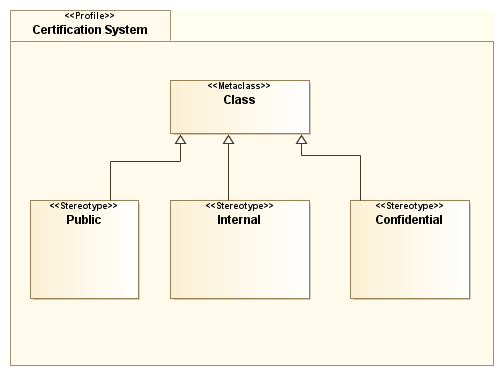
\includegraphics[scale=0.5]{uml/datastereotypes.png}
    \caption{Das Metamodell wird mit einem Profil um drei Stereotypen erweitert, welche die Zonen der Applikation darstellen}
\end{figure}

Zusätzlich werden diese Zonen auch mit Vertrautheitsebenen verbunden. Diese Ebenen werden im Profil mit einer Notiz versehen, welche die Ebene angibt.

\begin{figure}[H]
    \centering
    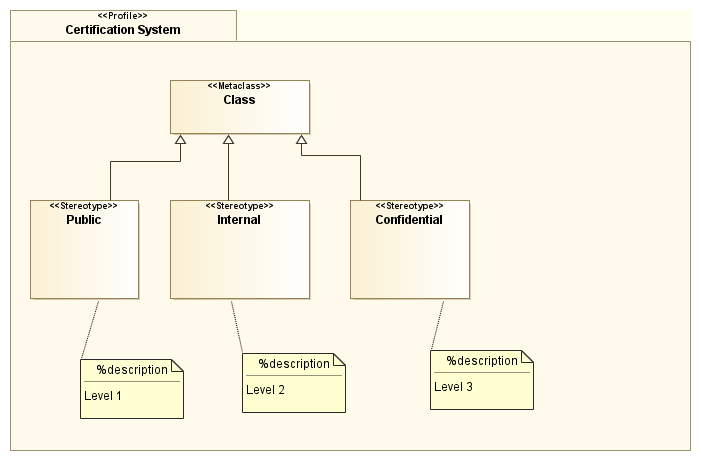
\includegraphics[scale=0.5]{uml/datastereotypeslevel.png}
    \caption{Die Zonen werden mit Vertrautheitsebenen versehen}
\end{figure}

Sind die Stereotypen erstellt und mit Vertrautheitsebenen versehen, kann nun damit begonnen werden, die AkteurInnen des Usecase Diagrammes und die Daten des Klassen Diagrammes mit diesen Stereotypen zu versehen.

\begin{figure}[H]
    \centering
    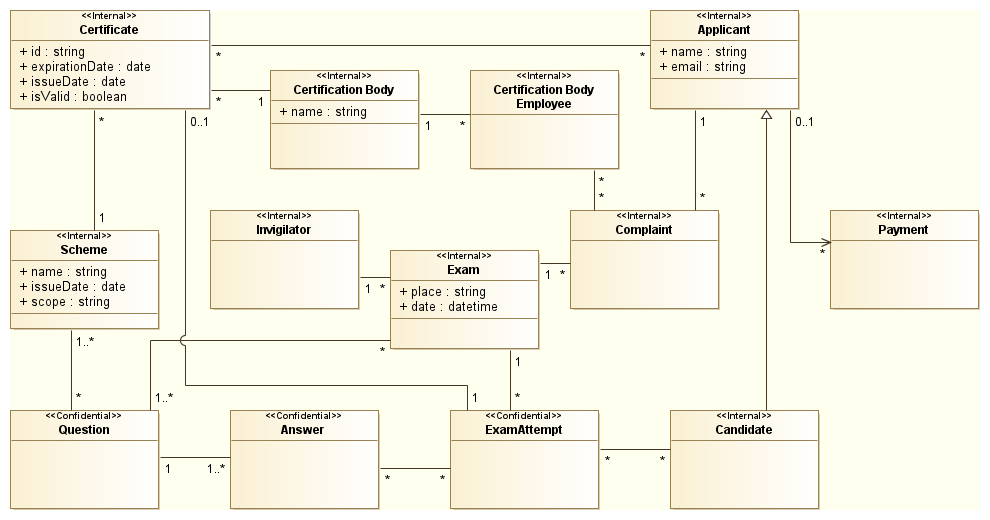
\includegraphics[scale=0.5]{uml/classstereotyped.png}
    \caption{Das Klassendiagramm wird mit Stereotypen der Vertraulichkeit erweitert}
\end{figure}

\begin{figure}[H]
    \centering
    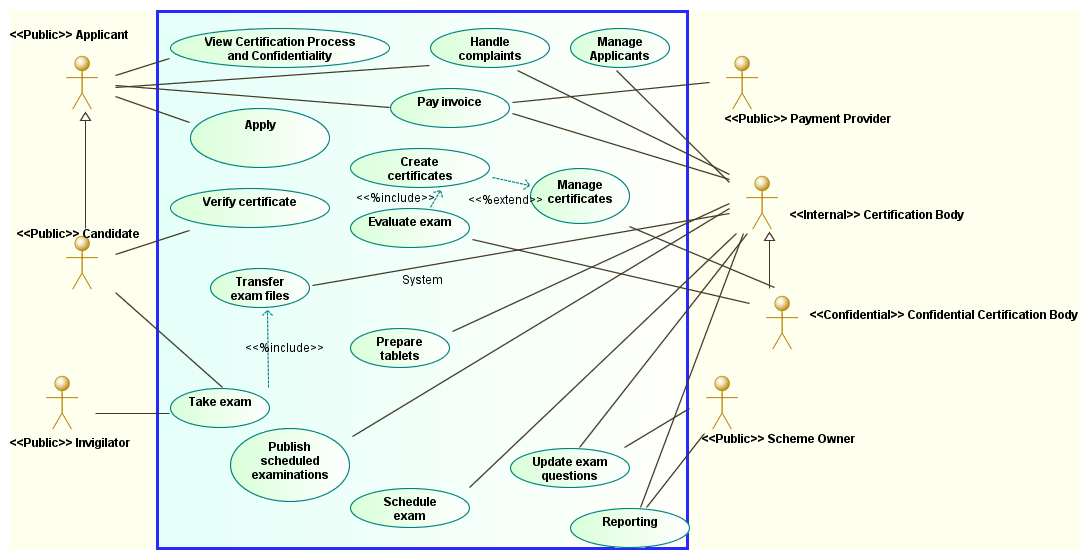
\includegraphics[scale=0.4]{uml/stereotypedusecase.png}
    \caption{Die AkteurInnen des Usecase Diagrammes wird mit Stereotypen der Vertraulichkeit erweitert}
\end{figure}

\section{Ermittlung der Beziehungen zwischen Akteuren/Partnersystemen und Daten}
Auf Basis des Usecase Diagrammes können die Akteure und deren Partnersysteme mit Hilfe eines Kontext Diagrammes visualisiert werden. Im Gegensatz zum Usecase Diagramm geht das Kontext Diagramm auf die zwischen den Systemen und AkteurInnen fließenden Daten ein und stellt so die Verbindung der Daten und Nutzer auf.

\begin{figure}[H]
    \centering
    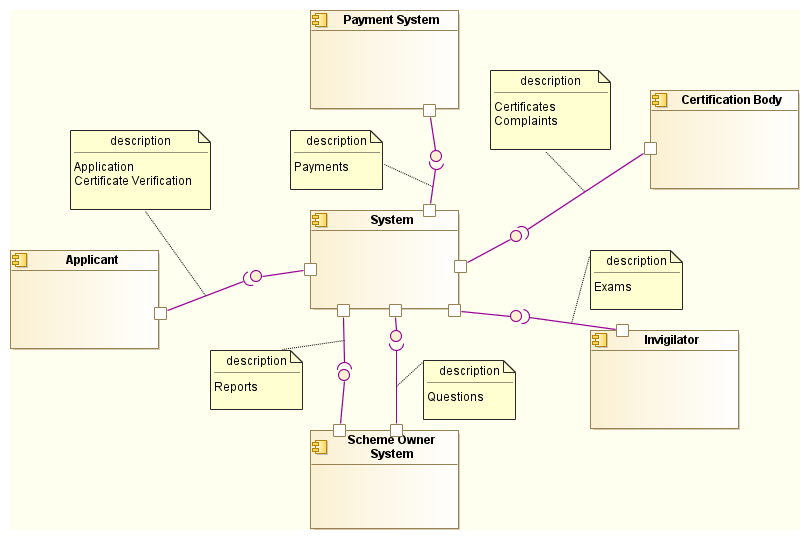
\includegraphics[scale=0.5]{uml/context.png}
    \caption{Das Kontext Diagramm zeigt das System, die Akteure und die Nachbarsysteme}
\end{figure}